% This contents of this file will be inserted into the _Solutions version of the
% output tex document.  Here's an example:

% If assignment with subquestion (1.a) requires a written response, you will
% find the following flag within this document: <SCPD_SUBMISSION_TAG>_1a
% In this example, you would insert the LaTeX for your solution to (1.a) between
% the <SCPD_SUBMISSION_TAG>_1a flags.  If you also constrain your answer between the
% START_CODE_HERE and END_CODE_HERE flags, your LaTeX will be styled as a
% solution within the final document.

% Please do not use the '<SCPD_SUBMISSION_TAG>' character anywhere within your code.  As expected,
% that will confuse the regular expressions we use to identify your solution.

\def\assignmentnum{6 }
\def\assignmentname{Bayesian Networks}
\def\assignmenttitle{XCS221 Assignment \assignmentnum --- \assignmentname}

\documentclass{article}
\usepackage[top = 1.0in]{geometry}

\usepackage{graphicx}

\usepackage[utf8]{inputenc}
\usepackage{listings}
\usepackage[dvipsnames]{xcolor}
\usepackage{bm}
\usepackage{algorithm}
\usepackage{algpseudocode}
\usepackage{framed}
\usepackage{wrapfig}
\usepackage{mathrsfs}

\definecolor{codegreen}{rgb}{0,0.6,0}
\definecolor{codegray}{rgb}{0.5,0.5,0.5}
\definecolor{codepurple}{rgb}{0.58,0,0.82}
\definecolor{backcolour}{rgb}{0.95,0.95,0.92}

\lstdefinestyle{mystyle}{
    backgroundcolor=\color{backcolour},   
    commentstyle=\color{codegreen},
    keywordstyle=\color{magenta},
    stringstyle=\color{codepurple},
    basicstyle=\ttfamily\footnotesize,
    breakatwhitespace=false,         
    breaklines=true,                 
    captionpos=b,                    
    keepspaces=true,                 
    numbersep=5pt,                  
    showspaces=false,                
    showstringspaces=false,
    showtabs=false,                  
    tabsize=2
}

\lstset{style=mystyle}

\newcommand{\di}{{d}}
\newcommand{\nexp}{{n}}
\newcommand{\nf}{{p}}
\newcommand{\vcd}{{\textbf{D}}}
\newcommand{\Int}{\mathbb{Z}}
\newcommand\bb{\ensuremath{\mathbf{b}}}
\newcommand\bs{\ensuremath{\mathbf{s}}}
\newcommand\bp{\ensuremath{\mathbf{p}}}
\newcommand{\relu} { \operatorname{ReLU} }
\newcommand{\smx} { \operatorname{softmax} }
\newcommand\bx{\ensuremath{\mathbf{x}}}
\newcommand\bh{\ensuremath{\mathbf{h}}}
\newcommand\bc{\ensuremath{\mathbf{c}}}
\newcommand\bW{\ensuremath{\mathbf{W}}}
\newcommand\by{\ensuremath{\mathbf{y}}}
\newcommand\bo{\ensuremath{\mathbf{o}}}
\newcommand\be{\ensuremath{\mathbf{e}}}
\newcommand\ba{\ensuremath{\mathbf{a}}}
\newcommand\bu{\ensuremath{\mathbf{u}}}
\newcommand\bv{\ensuremath{\mathbf{v}}}
\newcommand\bP{\ensuremath{\mathbf{P}}}
\newcommand\bg{\ensuremath{\mathbf{g}}}
\newcommand\bX{\ensuremath{\mathbf{X}}}
% real numbers R symbol
\newcommand{\Real}{\mathbb{R}}

% encoder hidden
\newcommand{\henc}{\bh^{\text{enc}}}
\newcommand{\hencfw}[1]{\overrightarrow{\henc_{#1}}}
\newcommand{\hencbw}[1]{\overleftarrow{\henc_{#1}}}

% encoder cell
\newcommand{\cenc}{\bc^{\text{enc}}}
\newcommand{\cencfw}[1]{\overrightarrow{\cenc_{#1}}}
\newcommand{\cencbw}[1]{\overleftarrow{\cenc_{#1}}}

% decoder hidden
\newcommand{\hdec}{\bh^{\text{dec}}}

% decoder cell
\newcommand{\cdec}{\bc^{\text{dec}}}

\newcommand{\expect}[1]{\noindent{\textbf{What we expect:} #1}}

\usepackage[hyperfootnotes=false]{hyperref}
\hypersetup{
  colorlinks=true,
  linkcolor = blue,
  urlcolor  = blue,
  citecolor = blue,
  anchorcolor = blue,
  pdfborderstyle={/S/U/W 1}
}
\usepackage{nccmath}
\usepackage{mathtools}
\usepackage{graphicx,caption}
\usepackage[shortlabels]{enumitem}
\usepackage{epstopdf,subcaption}
\usepackage{psfrag}
\usepackage{amsmath,amssymb,epsf}
\usepackage{verbatim}
\usepackage{cancel}
\usepackage{color,soul}
\usepackage{bbm}
\usepackage{listings}
\usepackage{setspace}
\usepackage{float}
\definecolor{Code}{rgb}{0,0,0}
\definecolor{Decorators}{rgb}{0.5,0.5,0.5}
\definecolor{Numbers}{rgb}{0.5,0,0}
\definecolor{MatchingBrackets}{rgb}{0.25,0.5,0.5}
\definecolor{Keywords}{rgb}{0,0,1}
\definecolor{self}{rgb}{0,0,0}
\definecolor{Strings}{rgb}{0,0.63,0}
\definecolor{Comments}{rgb}{0,0.63,1}
\definecolor{Backquotes}{rgb}{0,0,0}
\definecolor{Classname}{rgb}{0,0,0}
\definecolor{FunctionName}{rgb}{0,0,0}
\definecolor{Operators}{rgb}{0,0,0}
\definecolor{Background}{rgb}{0.98,0.98,0.98}
\lstdefinelanguage{Python}{
    numbers=left,
    numberstyle=\footnotesize,
    numbersep=1em,
    xleftmargin=1em,
    framextopmargin=2em,
    framexbottommargin=2em,
    showspaces=false,
    showtabs=false,
    showstringspaces=false,
    frame=l,
    tabsize=4,
    % Basic
    basicstyle=\ttfamily\footnotesize\setstretch{1},
    backgroundcolor=\color{Background},
    % Comments
    commentstyle=\color{Comments}\slshape,
    % Strings
    stringstyle=\color{Strings},
    morecomment=[s][\color{Strings}]{"""}{"""},
    morecomment=[s][\color{Strings}]{'''}{'''},
    % keywords
    morekeywords={import,from,class,def,for,while,if,is,in,elif,else,not,and,or
    ,print,break,continue,return,True,False,None,access,as,,del,except,exec
    ,finally,global,import,lambda,pass,print,raise,try,assert},
    keywordstyle={\color{Keywords}\bfseries},
    % additional keywords
    morekeywords={[2]@invariant},
    keywordstyle={[2]\color{Decorators}\slshape},
    emph={self},
    emphstyle={\color{self}\slshape},
%
}
\lstMakeShortInline|

\pagestyle{empty} \addtolength{\textwidth}{1.0in}
\addtolength{\textheight}{0.5in}
\addtolength{\oddsidemargin}{-0.5in}
\addtolength{\evensidemargin}{-0.5in}
\newcommand{\ruleskip}{\bigskip\hrule\bigskip}
\newcommand{\nodify}[1]{{\sc #1}}
\newenvironment{answer}{\sf \begingroup\color{ForestGreen}}{\endgroup}%

\setlist[itemize]{itemsep=2pt, topsep=0pt}
\setlist[enumerate]{itemsep=6pt, topsep=0pt}

\setlength{\parindent}{0pt}
\setlength{\parskip}{4pt}
\setlist[enumerate]{parsep=4pt}
\setlength{\unitlength}{1cm}

\renewcommand{\Re}{{\mathbb R}}
\newcommand{\R}{\mathbb{R}}
\newcommand{\what}[1]{\widehat{#1}}

\renewcommand{\comment}[1]{}
\newcommand{\mc}[1]{\mathcal{#1}}
\newcommand{\half}{\frac{1}{2}}

\DeclareMathOperator*{\argmin}{arg\,min}

\def\KL{D_{KL}}
\def\xsi{x^{(i)}}
\def\ysi{y^{(i)}}
\def\zsi{z^{(i)}}
\def\E{\mathbb{E}}
\def\calN{\mathcal{N}}
\def\calD{\mathcal{D}}
\def\slack{\url{http://xcs221-scpd.slack.com/}}
\def\zipscriptalt{\texttt{python zip\_submission.py}}
\DeclarePairedDelimiter\abs{\lvert}{\rvert}%
 
\usepackage{bbding}
\usepackage{pifont}
\usepackage{wasysym}
\usepackage{amssymb}
\usepackage{framed}
\usepackage{scrextend}

\newcommand{\alns}[1] {
	\begin{align*} #1 \end{align*}
}

\newcommand{\pd}[2] {
 \frac{\partial #1}{\partial #2}
}
\renewcommand{\Re} { \mathbb{R} }
\newcommand{\btx} { \mathbf{\tilde{x}} }
\newcommand{\bth} { \mathbf{\tilde{h}} }
\newcommand{\sigmoid} { \operatorname{\sigma} }
\newcommand{\CE} { \operatorname{CE} }
\newcommand{\byt} { \hat{\by} }
\newcommand{\yt} { \hat{y} }

\newcommand{\oft}[1]{^{(#1)}}
\newcommand{\fone}{\ensuremath{F_1}}

\newcommand{\ac}[1]{ {\color{red} \textbf{AC:} #1} }
\newcommand{\ner}[1]{\textbf{\color{blue} #1}}

% LLM Prompt box
\definecolor{llmpromptbg}{RGB}{235, 242, 255}
\newenvironment{llmprompt}{%
  \def\FrameCommand{\colorbox{llmpromptbg}}%
  \setlength\fboxsep{10pt}%
  \MakeFramed{\advance\hsize-\width \FrameRestore}%
  \noindent{\small\bfseries\color{RoyalBlue}Prompt Template}\par\smallskip%
  \small
}{%
  \endMakeFramed
}

% Red outline box (no header)
\definecolor{redoutline}{RGB}{200, 0, 0}
\newenvironment{redbox}{%
  \def\FrameCommand{\fcolorbox{redoutline}{white}}%
  \setlength\fboxsep{10pt}%
  \MakeFramed{\advance\hsize-\width \FrameRestore}%
}{%
  \endMakeFramed
}

\begin{document}
\pagestyle{myheadings} \markboth{}{\assignmenttitle}

% <SCPD_SUBMISSION_TAG>_entire_submission

This handout includes space for every question that requires a written response.
Please feel free to use it to handwrite your solutions (legibly, please).  If
you choose to typeset your solutions, the |README.md| for this assignment includes
instructions to regenerate this handout with your typeset \LaTeX{} solutions.
\ruleskip

\LARGE
1.a
\normalsize

% <SCPD_SUBMISSION_TAG>_1a
\begin{answer}
  % ### START CODE HERE ###
  \begin{center}
    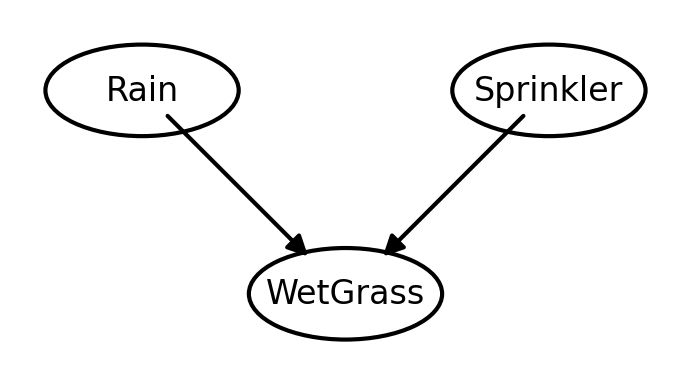
\includegraphics[width=0.45\textwidth]{images/1a-dag.png}
  \end{center}

  $\text{Rain} \rightarrow \text{WetGrass}$ and $\text{Sprinkler} \rightarrow \text{WetGrass}$.
  % ### END CODE HERE ###
\end{answer}
% <SCPD_SUBMISSION_TAG>_1a

\LARGE
1.b
\normalsize

% <SCPD_SUBMISSION_TAG>_1b
\begin{answer}
  % ### START CODE HERE ###
  The joint is the product of each variable's local conditional probability given its parents:
  \[
    \mathbb{P}(\text{Rain} = r, \text{Sprinkler} = s, \text{WetGrass} = w)
      = p(r)\, p(s)\, p(w \mid r, s) .
  \]
  % ### END CODE HERE ###
\end{answer}
% <SCPD_SUBMISSION_TAG>_1b

\LARGE
1.c
\normalsize

% <SCPD_SUBMISSION_TAG>_1c
\begin{answer}
  % ### START CODE HERE ###
  The sum the joint over both values of Rain and both values of Sprinkler:
  \[
    \mathbb{P}(\text{WetGrass} = w)
      = \sum_{r} \sum_{s} p(r)\, p(s)\, p(w \mid r, s) .
  \]
  % ### END CODE HERE ###
\end{answer}
% <SCPD_SUBMISSION_TAG>_1c

\LARGE
1.d
\normalsize

% <SCPD_SUBMISSION_TAG>_1d
\begin{answer}
  % ### START CODE HERE ###
  The grass is wet with probability 0.9 when it rained and the sprinklers were on, so it stays dry
  with probability $1 - 0.9 = 0.1$:
  \[
    \begin{aligned}
      \mathbb{P}(\text{Rain} = 1, \text{Sprinkler} = 1, \text{WetGrass} = 0)
        &= p(\text{Rain} = 1)\, p(\text{Sprinkler} = 1)\, p(\text{WetGrass} = 0 \mid \text{Rain} = 1, \text{Sprinkler} = 1) \\
        &= 0.2 \times 0.5 \times 0.1 = 0.01 .
    \end{aligned}
  \]
  % ### END CODE HERE ###
\end{answer}
% <SCPD_SUBMISSION_TAG>_1d

\LARGE
1.e
\normalsize

% <SCPD_SUBMISSION_TAG>_1e
\begin{answer}
  % ### START CODE HERE ###
  % Working for (c), kept for reference, not rendered:
  %   P(Rain, Wet)            = 0.2*0.5*0.9 + 0.2*0.5*0.8 = 0.09 + 0.08 = 0.17
  %   P(Wet)                  = 0.17 + 0.8*0.5*0.7 + 0.8*0.5*0.0 = 0.45
  %   P(Rain | Wet)           = 0.17 / 0.45 = 0.378
  %   P(Rain, Sprinkler, Wet) = 0.09
  %   P(Sprinkler, Wet)       = 0.09 + 0.28 = 0.37
  %   P(Rain | Wet, Sprinkler)= 0.09 / 0.37 = 0.243
  \begin{enumerate}[label=(\alph*)]
    \item True.
    \item False.
    \item True.
  \end{enumerate}
  % ### END CODE HERE ###
\end{answer}
% <SCPD_SUBMISSION_TAG>_1e
\clearpage

\LARGE
2.d
\normalsize

% <SCPD_SUBMISSION_TAG>_2d
\begin{answer}
  % ### START CODE HERE ###
  One run of \texttt{forward\_sampling} with \texttt{mutation\_rate = 0.1} and \texttt{genome\_length = 10}:

  \begin{center}
  \lstDeleteShortInline|
  \begin{tabular}{|l|l|}
  \hline
  \textbf{Species} & \textbf{Genome} \\
  \hline
  Thomas bayus & \texttt{TTCCATTCCC} \\
  Humblus studentus & \texttt{TGCCATTCCT} \\
  Aryamus bayus & \texttt{TTCCATTCCC} \\
  Kenius bayus & \texttt{TTCCATTCCC} \\
  \hline
  \end{tabular}
  \lstMakeShortInline|
  \end{center}
  % ### END CODE HERE ###
\end{answer}
% <SCPD_SUBMISSION_TAG>_2d

\LARGE
2.g
\normalsize

% <SCPD_SUBMISSION_TAG>_2g
\begin{answer}
  % ### START CODE HERE ###
  Estimates of $\mathbb{P}(\text{ThomasBayus} = \text{AAAC} \mid \text{KeniusBayus} = \text{AAAA})$,
  from \texttt{test\_gibbs\_vs\_rejection} with \texttt{mutation\_rate = 0.1}, \texttt{genome\_length = 4}, seed 0:

  \begin{center}
  \lstDeleteShortInline|
  \begin{tabular}{|l|c|l|}
  \hline
  \textbf{Method} & \textbf{Steps/Iterations} & \textbf{Estimated Posterior} \\
  \hline
  Rejection sampling & 100 & 0.0000 \\
  Rejection sampling & 10,000 & 0.0667 \\
  Gibbs sampling & 100 & 0.0900 \\
  Gibbs sampling & 10,000 & 0.0332 \\
  Exact & --- & 0.0335 \\
  \hline
  \end{tabular}
  \lstMakeShortInline|
  \end{center}
  % ### END CODE HERE ###
\end{answer}
% <SCPD_SUBMISSION_TAG>_2g
\clearpage

\LARGE
3.a
\normalsize

% <SCPD_SUBMISSION_TAG>_3a
\begin{answer}
  % ### START CODE HERE ###
  \begin{center}
    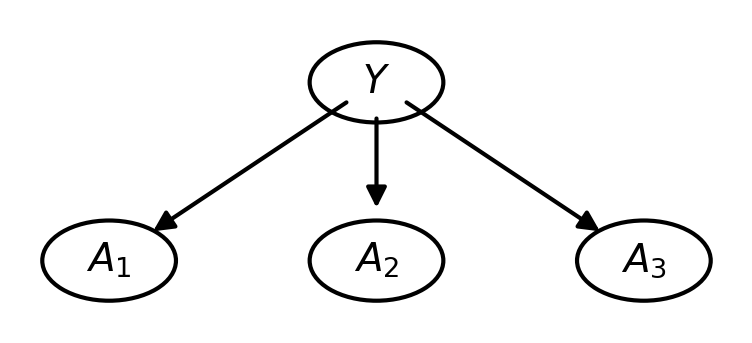
\includegraphics[width=0.45\textwidth]{images/3a-dag.png}
  \end{center}

  $Y \rightarrow A_1$, $Y \rightarrow A_2$ and $Y \rightarrow A_3$. Each annotator's label depends on
  the true label.
  % ### END CODE HERE ###
\end{answer}
% <SCPD_SUBMISSION_TAG>_3a

\LARGE
3.b
\normalsize

% <SCPD_SUBMISSION_TAG>_3b
\begin{answer}
  % ### START CODE HERE ###
  A perfect annotator gives the true label.

  \begin{center}
  \lstDeleteShortInline|
  \begin{tabular}{|c|c|c|}
  \hline
  $Y$ & $p(A_1 = \text{good} \mid Y)$ & $p(A_1 = \text{bad} \mid Y)$ \\
  \hline
  $\text{good}$ & 1 & 0 \\
  $\text{bad}$ & 0 & 1 \\
  \hline
  \end{tabular}
  \lstMakeShortInline|
  \end{center}
  % ### END CODE HERE ###
\end{answer}
% <SCPD_SUBMISSION_TAG>_3b

\LARGE
3.c
\normalsize

% <SCPD_SUBMISSION_TAG>_3c
\begin{answer}
  % ### START CODE HERE ###
  A random annotator gives exactly a random result.

  \begin{center}
  \lstDeleteShortInline|
  \begin{tabular}{|c|c|c|}
  \hline
  $Y$ & $p(A_1 = \text{good} \mid Y)$ & $p(A_1 = \text{bad} \mid Y)$ \\
  \hline
  $\text{good}$ & 0.5 & 0.5 \\
  $\text{bad}$ & 0.5 & 0.5 \\
  \hline
  \end{tabular}
  \lstMakeShortInline|
  \end{center}
  % ### END CODE HERE ###
\end{answer}
% <SCPD_SUBMISSION_TAG>_3c

\LARGE
3.g
\normalsize

% <SCPD_SUBMISSION_TAG>_3g
\begin{answer}
  % ### START CODE HERE ###
  \begin{center}
    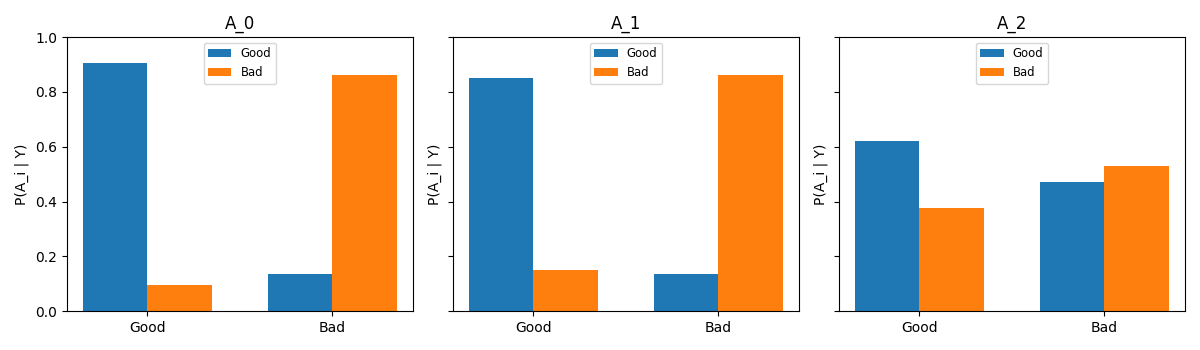
\includegraphics[width=\textwidth]{images/3g-annotator-cpts.png}
  \end{center}

  A\_2 is the least trustworthy. It is the least accurate been right about 62\% of the time when the label is good and 53\% for the label bad, so it is close to the random annotator. A\_0 and
  A\_1 are right around 85 to 90\% of the time.
  % ### END CODE HERE ###
\end{answer}
% <SCPD_SUBMISSION_TAG>_3g
\clearpage

\LARGE
4.d
\normalsize

% <SCPD_SUBMISSION_TAG>_4d
\begin{answer}
  % ### START CODE HERE ###
  Annotator tables after 100 iterations of EM on the unlabelled annotations:

  \begin{center}
    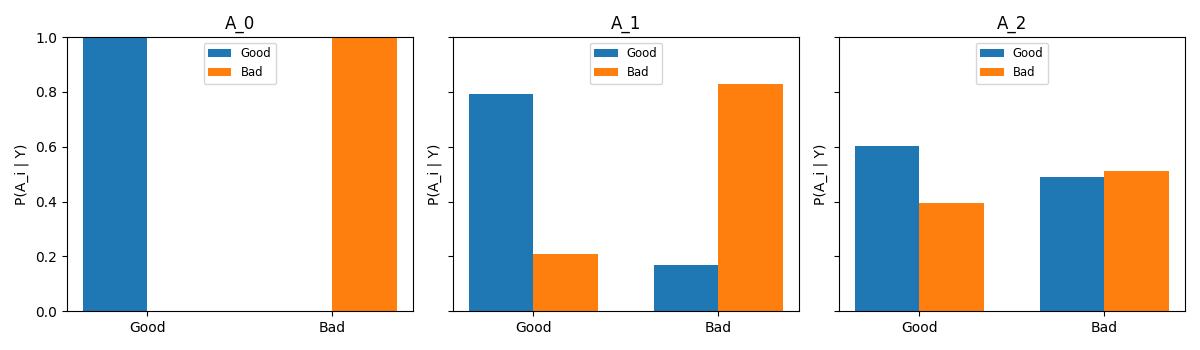
\includegraphics[width=\textwidth]{images/4d-annotators-em.png}
  \end{center}

  Estimated $P(\text{good})$ for each data point, split by its true label:

  \begin{center}
    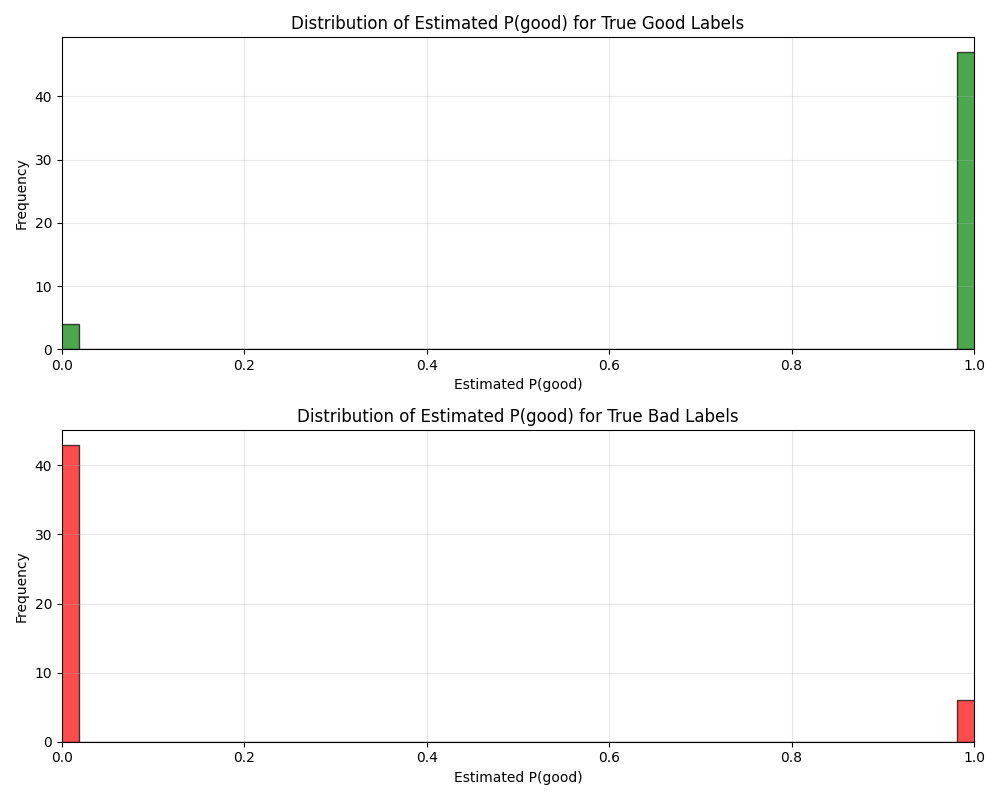
\includegraphics[width=0.8\textwidth]{images/4d-labels-em.png}
  \end{center}
  % ### END CODE HERE ###
\end{answer}
% <SCPD_SUBMISSION_TAG>_4d

\LARGE
4.e
\normalsize

% <SCPD_SUBMISSION_TAG>_4e
\begin{answer}
  % ### START CODE HERE ###
  % Checked against the labelled file: EM right 90/100, A_0 right 90/100,
  % EM agrees with A_0 on 100/100.
  The EM algorithm only recovered the true labels partly. About 90 of the 100 points end up on the right side. But the annotator plot shows EM turned A\_0 into a perfect annotator, so it really just learned A\_0's labels. That works here because A\_0 was the most accurate annotator in 3g, and the points EM
  gets wrong are the ones A\_0 got wrong.
  % ### END CODE HERE ###
  \end{answer}
% <SCPD_SUBMISSION_TAG>_4e

\clearpage


\LARGE
5.a
\normalsize

% <SCPD_SUBMISSION_TAG>_5a
\begin{answer}
  % ### START CODE HERE ###
  Claude Code is mostly used to automate programming tasks like adding features, writing tests and
  building small apps, so it matters most for software developers, especially front-end and web
  developers. Anthropic's own study found 79\% of Claude Code conversations were automation, against
  49\% on Claude.ai, with building user interfaces the most common use
  (\href{https://www.anthropic.com/research/impact-software-development}{Anthropic Economic Index,
  April 2025}). Startups adopted it first, with enterprises behind. Upstream it also depends on crowd
  workers who rate and safety-test the model, and on the developers and writers whose code and text
  are in the training data.
  % ### END CODE HERE ###
\end{answer}
% <SCPD_SUBMISSION_TAG>_5a

\LARGE
5.b
\normalsize

% <SCPD_SUBMISSION_TAG>_5b
\begin{answer}
  % ### START CODE HERE ###
  Claude Code is more likely to replace entry-level work and help experienced developers than to
  replace developers outright. Stanford's \textit{Canaries in the Coal Mine} study found employment
  for 22 to 25 year olds in AI-exposed jobs, software included, is 19\% below where it should be, while
  experienced workers show no gap
  (\href{https://digitaleconomy.stanford.edu/news/canariesaug26/}{Stanford Digital Economy Lab}). For
  workers the risk is that if companies stop hiring juniors, nobody becomes a senior later. For
  employers the risk is code nobody fully understands, since it can pass tests and still be wrong,
  which I ran into several times in this course.
  % ### END CODE HERE ###
\end{answer}
% <SCPD_SUBMISSION_TAG>_5b

\LARGE
5.c
\normalsize

% <SCPD_SUBMISSION_TAG>_5c
\begin{answer}
  % ### START CODE HERE ###
  Claude Code eappars to favour English-speaking, higher-income users. Because plans go from about \$17 a month to
  \$100--200 for Max, so richer users get stronger models and higher limits, and some regions can't
  use it at all. The Opus 5 system card says quality varies by language but only gives one average
  across 42 languages (92.5\%), and nothing for coding, so someone prompting in another language may
  get worse code without anyone seeing it. To improve transparency, Anthropic could publish Claude Code's success and error
  rates by prompt language and plan tier.
  % ### END CODE HERE ###
\end{answer}
% <SCPD_SUBMISSION_TAG>_5c

\LARGE
5.d
\normalsize

% <SCPD_SUBMISSION_TAG>_5d
\begin{answer}
  % ### START CODE HERE ###
  My proposed solution is companies could scale how much Claude Code does with how experienced the developer is. Juniors get
  low automation access, with Claude Code explaining instead of writing finished code, and high oversight,
  approving each action and getting their changes reviewed. As they gain experience oversight drops
  and automation goes up. Companies can continue to hire
  juniors developers since they are still productive with oversight, and they actually learn, so the pipeline from 5b doesn't
  dry up.
  % ### END CODE HERE ###
\end{answer}
% <SCPD_SUBMISSION_TAG>_5d
\clearpage

\LARGE
6.a
\normalsize

% <SCPD_SUBMISSION_TAG>_6a
\begin{answer}
  % ### START CODE HERE ###
  Claude Code is Anthropic's coding agent. It runs in the terminal or an IDE, reads a codebase, edits
  files, runs commands and makes commits. In my own
  use it added a feature and tests to an investment backtester, built an app from scratch. Anthropic publishes a system card for each model, a plain usage policy
  and threat reports. Its weaknesses are its closed form position on its model and data settings. The training default
  isn't stated, the data page is hard to find, and \texttt{/feedback} reports are kept for five years.
  Individual users get no copyright indemnity while businesses do, support is private, fairness
  testing only covers the chat model, and it puts entry-level developers most at risk.

  For privacy and accountability, I would state the training default and show it the first time
  Claude Code launches, add a per-session view of what was kept for training and when it gets
  deleted, and make reported issues public with a way for users to vote on fixes.

  For fairness and jobs, I would publish Claude Code's success and error rates by language and plan
  tier, offer a mode for juniors that starts with low automation and hands over more as they gain
  experience, and give individual users copyright protection or at least flag outputs that match
  licensed code.
  % ### END CODE HERE ###
\end{answer}
% <SCPD_SUBMISSION_TAG>_6a

\LARGE
6.b
\normalsize

% <SCPD_SUBMISSION_TAG>_6b
\begin{answer}
  % ### START CODE HERE ###
  Right now Anthropic decides how Claude Code changes, and the only outside groups with real leverages are
  courts and paying businesses. In the music publishers' case Anthropic agreed to keep its copyright
  guardrails while the case goes on, and businesses get protections individual users don't.
  Individual users can report through \texttt{/bug} and GitHub, but there are over 5,000 open issues,
  so they have almost no say. I think users should have real influence since their code, data and jobs
  are affected and they see the problems first. A public list of reported issues and what Anthropic
  did about them, with users voting on what gets fixed first, would give that feedback real weight.
  % ### END CODE HERE ###
\end{answer}
% <SCPD_SUBMISSION_TAG>_6b
\clearpage

% <SCPD_SUBMISSION_TAG>_entire_submission

\end{document}